\section{流形上的函数与场}
\label{sec:mfd-functions-fields}

切空间和余切空间都是逐点的对象。实际问题中更常见的是随点变化的量：球面上每一点的温度是一个实数，每一点的风速是一个切向量。前者是函数，后者是向量场，把每点的余切向量排在一起又得到协向量场。一条贯穿的界线是：同一点处的值可以相加，不同点处的场值属于不同的线性空间，不能直接比较。

\subsection{光滑函数}
\label{sec:mfd-smooth-functions}

球面上的高度函数$h(\bm y)=y_3$给每一点赋一个实数。要问它是否光滑，仍然把它写进坐标。由式~\eqref{eq:mfd-stereographic-inverse}，高度就是$\sigma_N^{-1}$的第三个分量，于是在北极图中
\begin{equation}
\hat h(\bm u)=h(\sigma_N^{-1}(\bm u))=\frac{\rho-1}{\rho+1},\qquad \rho=\lVert\bm u\rVert_2^2 .
\label{eq:mfd-height-north}
\end{equation}
同样地，记$\tilde\rho=\lVert\bm w\rVert_2^2$，在南极图中
\begin{equation}
\tilde h(\bm w)=\frac{1-\tilde\rho}{1+\tilde\rho}.
\label{eq:mfd-height-south}
\end{equation}
两个表达式都是分母为正的有理函数，所以$h$在每张图中都光滑。

\begin{definition}[流形上的光滑函数]
\label{def:mfd-smooth-function}
设$M$是光滑流形，可以带边界。函数$f:M\to\mathbb R$称为\term{光滑函数}（smooth function），若对每张坐标图$(U,\varphi)$，坐标表示$\hat f=f\circ\varphi^{-1}:\varphi(U)\to\mathbb R$光滑；边界处的光滑性按定义~\ref{def:mfd-smooth-halfspace}理解。全体光滑函数组成的集合记为$C^\infty(M)$。
\end{definition}

与曲线的情形一样，只需在一个图册的每张图中检查：另一张图中的坐标表示等于这里的坐标表示与一个光滑转移映射的复合。光滑函数的和、积、数乘仍光滑，因为坐标表示逐点相加、相乘。

\paragraph{函数的微分}
沿一条曲线观察函数，就得到函数值随时间的变化率。设$p$是内点，$\bm v=[\gamma]\in T_pM$。在图$\varphi$中，$f\circ\gamma=\hat f\circ(\varphi\circ\gamma)$，链式法则给出
\[
(f\circ\gamma)'(0)=\sum_{i=1}^n\frac{\partial\hat f}{\partial x_i}(\varphi(p))\,v_i .
\]
右端只依赖坐标速度$\bm v$，与等价类中代表曲线的选择无关，并且对$\bm v$是线性的。所以它定义了$T_pM$上的一个线性泛函，即一个余切向量。

\begin{definition}[函数的微分]
\label{def:mfd-function-differential}
设$f\in C^\infty(M)$，$p\in M$，$(U,\varphi)$是包含$p$的坐标图。$f$在$p$处的微分是余切向量
\begin{equation}
\mathrm df_p=\sum_{i=1}^n\frac{\partial\hat f}{\partial x_i}(\varphi(p))\,\mathrm dx_i|_p\ \in T_p^*M .
\label{eq:mfd-function-differential}
\end{equation}
对$\bm v\in T_pM$，记$\bm v f=\mathrm df_p(\bm v)$，称为$f$沿$\bm v$的方向导数。
\end{definition}

式~\eqref{eq:mfd-function-differential}用了坐标，需要检查它与图无关。在另一张图中，$\hat f=\tilde f\circ\tau$，其中$\tau$是转移映射。链式法则给出$\nabla\hat f=\bm J^\top\nabla\tilde f$，也就是
\[
\nabla\tilde f=\bm J^{-\top}\nabla\hat f .
\]
这正是余切向量系数的变换规则\eqref{eq:mfd-covector-change}，所以两张图给出同一个$\mathrm df_p$。这一论证不用曲线，因此在边界点处同样适用。

对坐标函数$x_i$本身，坐标表示是$\bm x\mapsto x_i$，偏导数为$\delta_{i,j}$，于是$\mathrm d(x_i)_p=\mathrm dx_i|_p$。这解释了对偶基的记号：$\mathrm dx_i|_p$就是坐标函数$x_i$在$p$处的微分。同样，把坐标基向量作用于函数，得到
\[
\partial_i|_pf=\frac{\partial\hat f}{\partial x_i}(\varphi(p)),
\]
也就是对坐标表示求偏导数。

方向导数满足乘积法则
\[
\bm v(fg)=f(p)\,\bm vg+g(p)\,\bm vf,
\]
因为坐标表示的偏导数满足这一法则。它还只依赖$f$在$p$附近的值：两个函数在$p$的某个邻域上相等，坐标表示在$\varphi(p)$附近相等，偏导数也相等。

\paragraph{球面高度函数的微分}
现在把微分在球面上算一遍，并在两张图中核对。对式~\eqref{eq:mfd-height-north}求偏导，利用$\hat h=1-2/(\rho+1)$，得到
\[
\frac{\partial\hat h}{\partial u_i}=\frac{4u_i}{(\rho+1)^2}.
\]
在$p=(0,\tfrac35,\tfrac45)$处，$\bm u=(0,3)$，$\rho=9$，分母为$100$，于是
\[
\mathrm dh_p=0\cdot\mathrm du_1|_p+\frac{12}{100}\,\mathrm du_2|_p .
\]
读数的含义是：沿$\partial_{u_1}|_p$运动时高度不变，沿$\partial_{u_2}|_p$运动时高度以速率$0.12$变化。前面算过，$\partial_{u_1}|_p$在$\mathbb R^3$中是水平速度$(\tfrac15,0,0)$，它确实不改变高度。

换到南极图。对式~\eqref{eq:mfd-height-south}求偏导，在$\bm w=(0,\tfrac13)$处，$\tilde\rho=\tfrac19$，
\[
\frac{\partial\tilde h}{\partial w_2}=\frac{-4w_2}{(1+\tilde\rho)^2}=-\frac{4}{3}\cdot\frac{81}{100}=-1.08 .
\]
用式~\eqref{eq:mfd-covector-change}从北极图的系数换算，$\bm J^{-\top}=\operatorname{diag}(9,-9)$，得到
\[
\operatorname{diag}(9,-9)\,(0,\ 0.12)^\top=(0,\ -1.08)^\top ,
\]
两种算法一致。图~\ref{fig:mfd-height-rotation}(a)(c)中的蓝圈是高度函数的等高线，标注的数字就是高度值。

\begin{BookInlineFigure}
  \centering
  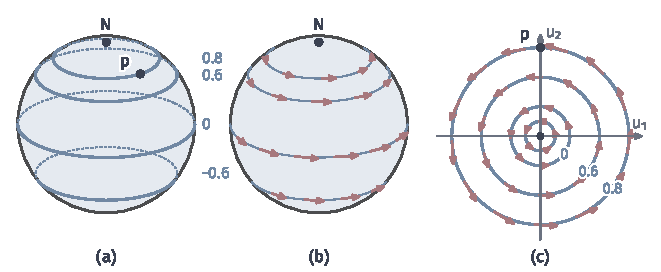
\includegraphics[width=112mm]{figures/04-spaces-measures-and-geometry/04-manifolds/matplotlib/mfd-height-rotation/figure.pdf}
  \caption{球面上的高度函数与旋转场。(a)蓝色纬线是$h=y_3$的等高线，右侧数字是高度，背面用虚线。(b)绕竖直轴的旋转场（红箭头）沿等高线切向，每点的箭头属于该点的切空间。(c)北极图中的同一组对象：半径$r$的圆对应高度$(r^2-1)/(r^2+1)$，半径$\tfrac12,1,2,3$的圆依次对应高度$-0.6,0,0.6,0.8$（最内圈未标数字），红箭头是分量$(-u_2,u_1)$的向量场，长度按比例缩小。}
  \label{fig:mfd-height-rotation}
\end{BookInlineFigure}

在北极，南极图坐标为$\bm w=\bm0$，$\tilde h$的偏导数在$\bm0$处都为零，所以$\mathrm dh_N=0$。这与极值的一般规律相符：若$f$在内点$p$处取局部最大值，则每条经过$p$的曲线$\gamma$使$f\circ\gamma$在$0$处取局部最大值，于是$\bm vf=(f\circ\gamma)'(0)=0$对所有$\bm v$成立，$\mathrm df_p=0$。球面紧，$h$的最大值一定取得，取在北极，微分在那里为零。

注意$\mathrm dh_p$是余切向量，不是一个“梯度方向”。要把它变成指向高度增加最快方向的切向量，需要在切空间上有内积，这一构造在第~\ref{chap:manifold-calculus}章完成。

\subsection{向量场与协向量场}
\label{sec:mfd-vector-covector-fields}

\paragraph{向量场}
设想球面绕竖直轴匀速旋转，每一点都有一个速度，它属于该点的切空间。把这些速度放在一起，就得到一个随点变化、每点取值在不同切空间中的对象，图~\ref{fig:mfd-height-rotation}(b)画的就是它。

\begin{definition}[光滑向量场]
\label{def:mfd-vector-field}
$M$上的\term{向量场}（vector field）$X$给每个$p\in M$指定一个切向量$X_p\in T_pM$。在坐标图$(U,\varphi)$中写成
\begin{equation}
X_p=\sum_{i=1}^nX_i(p)\,\partial_i|_p,\qquad p\in U,
\label{eq:mfd-vector-field-components}
\end{equation}
函数$X_i:U\to\mathbb R$称为$X$的分量。若在每张坐标图中分量都光滑，则称$X$为光滑向量场。$M$上全体光滑向量场的集合记为$\mathfrak X(M)$。
\end{definition}

两张图重叠处，分量按式~\eqref{eq:mfd-tangent-change}逐点变换：
\begin{equation}
\tilde X_k=\sum_{j=1}^n\frac{\partial\tilde x_k}{\partial x_j}\,X_j .
\label{eq:mfd-vector-field-change}
\end{equation}
转移映射的偏导数是光滑函数，所以一张图中分量光滑，另一张图中分量也光滑，只需在一个图册中检查。反过来，若在一个图册的每张图中给定一组光滑函数，并在每个重叠处满足式~\eqref{eq:mfd-vector-field-change}，它们就拼成一个光滑向量场。

\paragraph{协向量场}
同样地，给每点指定一个余切向量，就得到\term{协向量场}（covector field）$\omega$。在图中写成$\omega_p=\sum_ia_i(p)\,\mathrm dx_i|_p$，分量光滑时称为光滑协向量场，重叠处的系数按式~\eqref{eq:mfd-covector-change}变换。最重要的例子是光滑函数的微分：$\mathrm df$在图中的分量是$\partial\hat f/\partial x_i$，光滑，所以$\mathrm df$是光滑协向量场。

\paragraph{例子：球面的旋转场}
绕竖直轴转角$t$的旋转把$\bm y$送到
\[
(y_1\cos t-y_2\sin t,\ y_1\sin t+y_2\cos t,\ y_3),
\]
它不改变$y_3$。由式~\eqref{eq:mfd-stereographic-north}，北极图坐标$\bm u=(y_1,y_2)/(1-y_3)$随之做同一个平面旋转。对$t$在$0$处求导，旋转场在北极图中的分量为
\begin{equation}
(X_1,X_2)=(-u_2,\ u_1).
\label{eq:mfd-rotation-north}
\end{equation}
同理，在南极图中分量为$(-w_2,w_1)$，北极$\bm w=\bm0$处场值为零，这是绕轴旋转时轴上的点不动。

用式~\eqref{eq:mfd-vector-field-change}核对两组分量相容。由式~\eqref{eq:mfd-inversion-jacobian}，先注意$\bm u^\top(-u_2,u_1)^\top=0$，于是
\[
\bm J_\tau(\bm u)\begin{bmatrix}-u_2\\u_1\end{bmatrix}
=\frac{1}{\rho}\begin{bmatrix}-u_2\\u_1\end{bmatrix}.
\]
而$\bm w=\bm u/\rho$，右端恰是$(-w_2,w_1)$。两组分量拼成整个球面上的光滑向量场。

\paragraph{向量场作用于函数}
向量场与函数配合，逐点取方向导数，得到一个新函数：
\begin{equation}
(Xf)(p)=X_pf=\mathrm df_p(X_p).
\label{eq:mfd-field-on-function}
\end{equation}
在坐标图中，$Xf=\sum_iX_i\,\partial\hat f/\partial x_i$。$X$与$f$都光滑时，$Xf$光滑。映射$f\mapsto Xf$是线性的，并满足$X(fg)=f\,Xg+g\,Xf$。

例如旋转场作用于高度函数。由上一小节的偏导数，
\[
Xh=-u_2\cdot\frac{4u_1}{(\rho+1)^2}+u_1\cdot\frac{4u_2}{(\rho+1)^2}=0 .
\]
这符合直观：绕竖直轴旋转不改变高度。图~\ref{fig:mfd-height-rotation}(c)中红箭头沿等高线走，说的是同一件事。

\paragraph{场的逐点运算与不同点的比较}
同一点处的场值属于同一个切空间，所以$X+Y$、$gX$（$g$为光滑函数）可以逐点定义，结果仍是光滑向量场。不同点处的场值却属于不同的切空间，差$X_p-X_q$没有意义。用坐标分量相减看似可行，但结果依赖所选的图。

下面用一个具体计算说明这一点。在北极图中取常值分量的场$X=\partial_{u_1}$，定义在$S^2\setminus\{N\}$上。取$p=\sigma_N^{-1}(0,3)$与$q=\sigma_N^{-1}(1,0)=(1,0,0)$，北极图中两点处的分量都是$(1,0)$，相减为零，看起来是“同一个向量”。

换到南极图。由式~\eqref{eq:mfd-inversion-jacobian}，在$q$处$\bm J_\tau(1,0)=\operatorname{diag}(-1,1)$，于是两点处的分量分别是
\[
p:\ \bm J_\tau(0,3)(1,0)^\top=(\tfrac19,\ 0),\qquad
q:\ \bm J_\tau(1,0)(1,0)^\top=(-1,\ 0).
\]
两者之差不为零。可见“两个不同点处的切向量是否相同”没有与图无关的答案。比较不同点的方向需要额外的搬运规则，这是第~\ref{chap:riemannian-geometry}章联络与平行移动的任务。

\subsection{向量场的Lie括号}
\label{sec:mfd-lie-bracket}

向量场可以先后作用于函数。$Y$作用于$f$得到函数$Yf$，$X$再作用得到$X(Yf)$，交换次序得$Y(Xf)$。在欧氏空间中，常系数的偏导数可以交换次序；系数随点变化时，两种次序一般不同。这个差既不依赖度量，也有清楚的运动含义。

\paragraph{交换差仍是向量场}
两个一阶导数的复合本来是二阶算子，先写出来看。在坐标中记$X=\sum_iX_i\partial_i$，$Y=\sum_jY_j\partial_j$，$\hat f$为$f$的坐标表示，由乘积法则，
\[
X(Yf)=\sum_{i,j}X_i\,(\partial_iY_j)\,\partial_j\hat f+\sum_{i,j}X_iY_j\,\partial_i\partial_j\hat f .
\]
$Y(Xf)$的展开相同，只是$X,Y$对调。二阶偏导数可交换，两式中的二阶项相同，相减时抵消，只剩一阶项：
\begin{equation}
X(Yf)-Y(Xf)=\sum_{j=1}^n\Bigl(\sum_{i=1}^n\bigl(X_i\,\partial_iY_j-Y_i\,\partial_iX_j\bigr)\Bigr)\partial_j\hat f .
\label{eq:mfd-lie-bracket-coordinates}
\end{equation}
右端是某个向量场作用于$f$的结果，它的分量是括号中的光滑函数。

\begin{definition}[Lie括号]
\label{def:mfd-lie-bracket}
对$X,Y\in\mathfrak X(M)$，由
\begin{equation}
[X,Y]f=X(Yf)-Y(Xf)
\label{eq:mfd-lie-bracket-def}
\end{equation}
确定的向量场$[X,Y]$称为$X$与$Y$的\term{Lie括号}（Lie bracket）。在坐标图中，它的分量由式~\eqref{eq:mfd-lie-bracket-coordinates}给出。
\end{definition}

还要说明不同图中的分量拼成同一个向量场。在图$\varphi$中把式~\eqref{eq:mfd-lie-bracket-coordinates}定义的场记为$Z$，在图$\psi$中记为$\tilde Z$。二者在重叠处作用于任意光滑函数，都等于与图无关的$X(Yf)-Y(Xf)$。

把$f$取为第二张图的坐标函数$\tilde x_k$（只在重叠的开集上用，方向导数只依赖函数在点附近的值），得到
\[
\tilde Z_k=Z\tilde x_k=\sum_{j=1}^n Z_j\,\frac{\partial\tilde x_k}{\partial x_j},
\]
这正是变换规则\eqref{eq:mfd-vector-field-change}。

\paragraph{一个计算例子}
在$\mathbb R^2$上取$X=\partial_1$，$Y=x_1\partial_2$。由式~\eqref{eq:mfd-lie-bracket-coordinates}，$[X,Y]$的第二个分量是$X_1\partial_1Y_2=1$，其余为零，所以
\[
[X,Y]=\partial_2 .
\]
对函数直接核对。两种先后次序分别是
\[
X(Yf)=\partial_1(x_1\partial_2f)=\partial_2f+x_1\partial_1\partial_2f,\qquad
Y(Xf)=x_1\partial_2\partial_1f .
\]
相减得$\partial_2f$，与上面一致。

这个结果可以从运动的角度理解。沿$X$走时间$\varepsilon$是向右平移$\varepsilon$；沿$Y$走时间$\varepsilon$是把$(a,b)$变为$(a,b+\varepsilon a)$，向上移动的距离取决于当时的横坐标。从$(a,b)$出发，两种走法的终点分别是
\[
\text{先}X\text{后}Y:\ (a+\varepsilon,\ b+\varepsilon a+\varepsilon^2),\qquad
\text{先}Y\text{后}X:\ (a+\varepsilon,\ b+\varepsilon a).
\]
两条路线的终点相差$(0,\varepsilon^2)$，是二阶小量，方向正是$\partial_2$。Lie括号度量的就是两种运动先后次序不可交换的程度，图~\ref{fig:mfd-lie-bracket}画出了这两条路线。

\begin{BookInlineFigure}
  \centering
  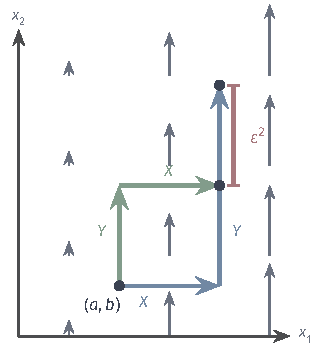
\includegraphics[width=54.906mm]{figures/04-spaces-measures-and-geometry/04-manifolds/tikz/mfd-lie-bracket/figure.pdf}
  \caption{Lie括号是运动次序的差。灰色箭头是场$Y=x_1\partial_2$，越往右越长。从$(a,b)=(1,\tfrac12)$出发，取$\varepsilon=1$：蓝色路线先沿$X=\partial_1$再沿$Y$，绿色路线先沿$Y$再沿$X$，终点相差红色线段$\varepsilon^2=1$，方向是$[X,Y]=\partial_2$。蓝色路线走$Y$时横坐标已经变大，所以走得更高。}
  \label{fig:mfd-lie-bracket}
\end{BookInlineFigure}

\paragraph{基本性质}
由定义直接可得反对称性与线性，对实数$a,b$和光滑函数$g$有
\[
\begin{gathered}
[X,Y]=-[Y,X],\qquad [aX+bY,Z]=a[X,Z]+b[Y,Z],\\
[X,gY]=g[X,Y]+(Xg)Y .
\end{gathered}
\]
此外还有Jacobi恒等式
\[
[X,[Y,Z]]+[Y,[Z,X]]+[Z,[X,Y]]=0,
\]
把三项都作用于$f$并按定义展开，得到十二个三阶复合项，它们两两抵消。坐标基向量场的Lie括号为零，$[\partial_i,\partial_j]=0$，这正是二阶偏导数可交换。

Lie括号的定义只用到向量场作用于函数，不需要先选度量或联络。第~\ref{chap:riemannian-geometry}章用它表述联络的无挠条件与曲率，第~\ref{chap:lie-groups}章用它刻画连续变换群在单位元附近的结构。
